\documentclass[a4paper,authorinfo]{handout}
\usepackage[latin1]{inputenc}
\usepackage{hyperref}
\usepackage{mathptm}

\course{http://www.es.oersted.dtu.dk/$\sim$sn/hpage}
\handoutnumber{}
\title{Short User's Guide to H-PaGe}
\author{Svetoslav Nikolov}
\address{�rsted$\bullet$DTU}
\logo{.figures/hpage_logo.pdf}

\release{1}

\newcommand{\hpage}{\textsf{H-PaGe}}
\newcommand{\menu}[1]{\emph{\underline{#1}}}


\begin{document}
\maketitle
\pagestyle{fancy}



\section{Introduction}
This is a short User's Guide for the \textbf{\sffamily H}ome \textbf{\sffamily Pa}ge \textbf{\sffamily Ge}nerator
(\textbf{\sffamily H-PaGe}, pronounced Eit$\int$ Peidzh).
\hpage  is a program which generates automatically
web pages from a given specification, which look
like the web pages of DTU. The user provides
only the \emph{content} of the page, and the layout
is created by \hpage. Thus, if the outer appearance
of the web site changes, the user can update his/her
web site without changing anything from his/her
files. This will be done automatically by \hpage.
The program was initially written to provide
a fast and easy way of creating and maintaining
web pages. Then some additional features have
been added to the program to make it more
flexible and usable.  Section \ref{sec: quick_start}
shows how to quickly and easy create  a web page.


\section{Quick Start}
\subsection{Creating a ``simple'' page}
\label{sec: quick_start}
\begin{figure}
\begin{center}
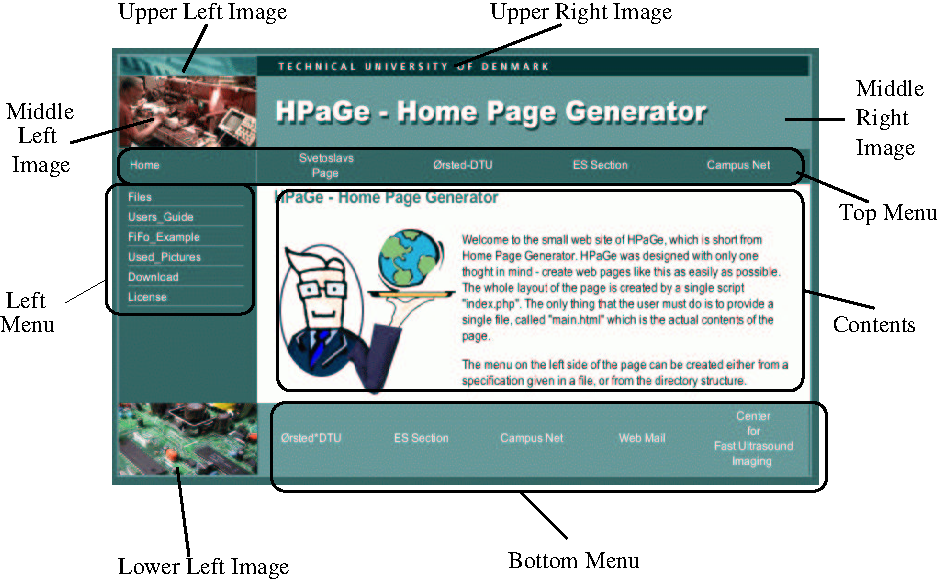
\epsfig{file=.figures/page_parts.pdf}
\caption{\label{fig: page_parts} Layout of the page generated
by \hpage.}
\end{center}
\end{figure}

\hpage~ creates pages like the one shown in Fig.~\ref{fig: page_parts}.
In order to create such a page, follow these steps:
\begin{enumerate}
\item Copy the file \code{index.php} to the directory which
      is going to be the \emph{root} directory of your
      web site. The file \code{index.php} is a small
      program written in PHP, which is executed by
      the web server. The output of the
      program is an HTML code for the page you will see  in
      your browser. Changing \code{index.php} will change
      the layout of the web page.

\item Copy the file \code{web.config} to the same directory.
      This file contains the names of the pictures which
      will appear in the web page. Presently it
      is necessary to provide names for at least
      4 pictures - upper-left, upper-right, middle-left,
      and middle-right (see Fig.~\ref{fig: page_parts}).

\item Create a file with a name \code{main.html}. This
file should be either a simple text file, or a simple
HTML file. The contents of this file will appear in
the middle row, on the left of the web page (the
one designated as ``Contents'' in Fig.~\ref{fig: page_parts}).
\end{enumerate}

\subsection{Playing With The Menus}
\label{sec: menus}
Consider again Fig.~\ref{fig: page_parts}.
Presently there are 3 menus, which are supported by
\hpage - left, top, and bottom menus. The top
and the bottom menus are optional. You can
choose either to have such menus, or not.
The left menu, however will always be present.
There are two ways of adding menu items
to the left menu: (a) using the directory
structure, and (b) using the file \code{web.config}.

\subsubsection{Adding menu items to the left menu}
The first way to add new items to the left menu
is to create new directories. For example,
let's assume that the file \code{index.php} is
placed in the directory \code{test}.
If now you create the following subdirectories of \code{test}:
\begin{quote}
\begin{verbatim}
Introduction
Test
.pictures
\end{verbatim}
\end{quote}
you will get two menu items in the left menu: \menu{Test} and
\menu{Introduction}. Directories, whose names start with
a \emph{dot} will be ``\emph{hidden}''.
Now, if you want to add some contents for these
two menu items, you must create two files \code{menu.html}
in \code{Introduction}, and \code{Test}, respectively.
When you click on the menu item \menu{Test}, then
the program will display the contents of the
file \code{Test/menu.html}.
If you want to add sub-menu items to the
menu items, then you must create sub-sub-directories
of the sub-directories. There is no limit
for the number of levels of sub-directories.
The recursion will, however, be stopped
if there is a file \code{index.php} in
some of the sub-directories. This way
of adding contents to your web site is
the simplest.

There is also another possibility for controlling
the contents of the menus - by changing the
file \code{web.config}


\subsubsection{Changing the menus from web.config}
It is possible to control the contents of
all of the menus from the file \code{web.config}.
The syntax of the command is:
\begin{quote}
\begin{verbatim}
add_menu('position', 'name', 'place', 'content');
\end{verbatim}
\end{quote}
where \code{position} specifies to which menu
an item is being added, and can be one of \code{'left'},
\code{'top'}, \code{'bottom'}. Notice that the
quotes (\code{\'}) are obligatory. So is the
semicolon (\code{;}) at the end of the line.
The second argument \code{'name'} is the
text that will appear on the screen. This can
be any valid HTML text. The third argument \code{'place'}
is the link itself. If \code{'place'} begins
with ``\code{http://}'', this means that the place is
an absolute Internet address. Otherwise, it is assumed
to be the name of a directory.  The last argument
\code{'content'} is optional.  It is used only
if \code{'place'} specifies a sub-directory.  The
default value of \code{'content'} is \code{'main.html'}.
Let's consider the following example.
We have created the two subdirectories
\code{Test}, and \code{Introduction}, and
we have the following file structure:
\begin{verbatim}
test/main.html
Introduction/main.html
Introduction/intro.html
Test/main.html
Test/test.html
\end{verbatim}
We can add items to the left menu using the following
commands:
\begin{verbatim}
add_menu('left','Main<br>Introduction', './Introduction');          # Line 1
add_menu('left','Some<br>Introduction', './Introduction','intro');  # Line 2
add_menu('left',"Test's test",'./Test');                            # Line 3
add_menu('left','<font color=yellow>Yellow<br>Test</font>','./Test','test.html');
add_menu('left','DTU','http://www.dtu.dk');                         # Line 5

\end{verbatim}
Several features have been demonstrated above.
You can have comments in your configuration. The comments
start with the letter \code{\#} and end with the end of line.
You can use double quotes (\code{"}) for the text, if you
have to use the single (\code{'}) quotes in the text. You can
use HTML tags to format your text. For example \code($<$br$>$)
breaks the line. The example on line 4, shows how you can even
change the color of a single link.

The link defined in line 1 will point to the file: \code{Introduction/main.html}
(\code{main.html} is the default file to be displayed).
The link in line 2 will point to the file \code{Introduction/intro.html}.
The script automatically checks for files \code{intro},
\code{intro.html} and \code{intro.htm}. Line 5 shows how
an absolute link is provided - placing \code{'http://'} in front of
the name.

Adding menu items to the top and bottom menus is done
in exactly the same way- just replacing the first
argument from \code{'left'} to \code{'top'} or \code{'bottom'},
respectively. If you do not add any items to the top and
bottom menus, they will not appear on the web page.
If you do not add any items to the left menu using
the command \code{add\_menu}, then the items
will be taken from the directory structure.


\subsection{Changing the pictures}
\label{sec: pictures}

Presently, there are at least 4 pictures
on the DTU web pages: upper-left, upper-right,
middle-left and middle-right (see Fig.~\ref{fig: page_parts}).
Optionally you can specify a bottom-left picture.
Adding the pictures to the page is done again
from the file \code{web.config} using the command:
\begin{quote}
\begin{verbatim}
add_image('position', 'file', 'description', 'link');
\end{verbatim}
\end{quote}
The first argument \code{'position'} is a string and
can take the following values: \code{'upperleft'},
\code{'upperright'}, \code{'middleleft'}, \code{'middleright'},
\code{'lowerleft'}, and {\code{'menu\_line'}}. The special picture
\code{'menu\_line'} is used for the line between the
items of the left menu. The second argument \code{'file'}
contains the path to the picture. The path is
given relative to the \emph{root} directory (the directory in
which \code{index.php} is placed). \code{'description'} is
a description of the picture. It is also shown
instead of the picture, if the picture cannot be displayed.
The last parameter \code{'link'} is optional.
If it exists, then the picture is used also as a link.
The link must be a full Internet address.


The sizes of the pictures is as follows:
\begin{itemize}
\item Upper-left  : 151 $\times$ 20 pixels.
\item Upper-right : 600 $\times$ 20 pixels.
\item Middle-left : 151 $\times$ 72 pixels.
\item Middle-right: 600 $\times$ 72 pixels.
\item Bottom-left : 151 $\times$ 72 pixels.
\end{itemize}

\emph{It is important that the images have
exactly this size, else a white spacing will
be added around them.
}

\subsection{Setting the title of the page}
\label{sec: title}
You can set a title for the web site using
the command:
\begin{quote}
\begin{verbatim}
set_title('text');
\end{verbatim}
\end{quote}

If you do not specify a middle-right image, then
the \code{text} for the title will be shown instead of
the middle-right picture.


\subsection{Adding a text at the bottom of the page}
\label{sec: add_text}

If you do not have a menu at the bottom of the page,
then you can have add a text at the bottom of the page
with the command \verb+add_bottom_text+. For example:
\begin{quote}
\begin{verbatim}
add_bottom_text('This page is maintained by <b>Svetoslav Nikolov</b>');
\end{verbatim}
\end{quote}


\subsection{Last updated ...}
If you want to show when a page was last
updated you can call the command \verb+show_updated+
with a parameter \verb+'true'+:
\begin{quote}
\begin{verbatim}
show_updated('true');
\end{verbatim}
\end{quote}

\subsection{Changing "Home"}
{\tt index.php} creates a default menu entry "Home",
which is the "Home" of the web site. If you 
want to change this text, for example to "Home MyName",
then you can use the command \verb+set_home_text('Some text')+:
\begin{quote}
\begin{verbatim}
set_home_text('H-PaGe Home');
\end{verbatim}
\end{quote}

\subsection{Changing The Color}
\label{sec: colors}
The contents of the web page must be structured.
For example you should specify: "this is a link",
"this is a header", etc. The colors and the fonts
are automatically controlled by the means
of "Cascaded Style Sheets" (CSS). They
are given in a separate file. You can
change the file with the CSS by using
the command:
\begin{quote}
\begin{verbatim}
set_style('file');
\end{verbatim}
\end{quote}
where \code{'file'} is the name of the file with CSS.
There are several such files, which can
be found in the distribution.  They have an extension
"\code{*.css}". You can get the decorations
for the different color schemes from the web.
The images are located in the subdirectory
\code{.pictures} of the distribution.


\section{Keeping everything in one single directory}
\label{sec: central}

When new versions of \code{index.php}
appear, you can update your web site
by copying it to the respective directories.
Alternatively, you can have only a
single copy of THE "\code{index.php}" in a
single directory, and in each directory you can have
a small file with the same name ("\code{index.php}"),
with the following text:
\begin{listing}
\code{$<$?php}\\
\code{~~~~include("/home/sn/2www/hpage/index.php");}\\
\code{?$>$}\\
\end{listing}
You must replace the path \verb+/home/sn/2www/hpage/+  with the path to
your own copy of  \code{index.php}.

\section{Additional Features}
\label{sec: additional}
The additional features are available only at �srsted$\bullet$DTU. They
include password protected directories and access to the publication
database.

\subsection{Accessing the publication database}
If \hpage{} opens a file with \verb+.php+ extension, it assumes
that the file is a script that has to be executed. A php script
is embedded in an HTML document like this:
\begin{verbatim}
Normal html document ....
<?
 PHP script - call commands from PHP
?>
Normal html document again ....
\end{verbatim}

\hpage{} provides a couple of useful function that you can use.
Let's assume that you want to show your publications in the
file \verb+publications.php+. The file will contain a fragment
of code like this:
\begin{verbatim}
<?
   pubdb_page(12, "conference", 2002, "Svetoslav's Conference papers");
?>
\end{verbatim}
The function \verb+pubdb_page+ connects to the publication database
of the department, retrieves the publications and displays them.
The function is defined as:
\begin{verbatim}
function pubdb_page($user_id=0, $type="all", $year="", $title="Publications")
\end{verbatim}
The inputs are \verb+user_id+, \verb+type+, \verb+year+, and \verb+title+.
\verb+user_id+ is the identification of the user. You can see it when 
you log in to the database. You can get your user ID either from 
Allan J�rgen, \verb+aj@oersted.dtu.dk+, or from Mogens Yndal Pedersen, \verb+myp@oersted.dtu.dk+.
The second parameter is the type of publications. It is a text string, 
and get one of the following values:
\begin{description}
\item{all}  - Show all publications
\item{journal} - Journal papers
\item{conference} - Conference papers
\item{book} - Book
\item{msc} - MSc Thesis
\item{phd } - PhD Thesis
\item{report} - Technical report
\item{notes} - Lecture note
\item{software} - Software
\item{misc} -  Misc
\item{patent} - Patent
\item{dsc} - Doctor thesis
\end{description}
The third parameter is \verb+year+. If you do not specify a year, then
all years will be included. The final parameter $title$ specifies
the title that should stay above the publications. 
The default value is "Publications".


If you want just to show a link to the publications database,
then you can use the functon \verb+pubdb_link+:
\begin{verbatim}
function pubdb_link($user_id, $type, $year, $title, $link_text)
\end{verbatim}
The only new paramater is \verb+link_text+, which is the text shown
as a link in you page.

\subsection{Password protection}
\label{sec: password}
If you want to restrict the access to some of your files,
you can add the command:
\begin{verbatim}
<?
 allow_users('sn','jaj', .....);
?>
\end{verbatim}
to your \verb+web.config+ file. The users will have to log in with
their login names for the web server. The transactions will
be done in sequre mode. Notice, that if you want to restrict
the access to information to only one of the subdirectories of
your web site, then the command \verb+allow_users+ must 
be placed in a file called \verb+web.addconfig+ in the respective
directory.


\end{document}
